\documentclass{lecture}

\institute{Lehrstuhl für Strömungslehre und Aerodynamisches Institut}
\title{Vorlesung 7}
\author{Joshua Feld, 406718}
\course{Strömungsmechanik I}
\professor{Schröder}
\semester{Sommersemester 2022}
\program{CES (Bachelor)}

\begin{document}
    \maketitle


    \section*{Strömung in offenen Gerinnen}
    
    Trotz vieler Gemeinsamkeiten mit der Strömung in geschlossenen Rohrleitungen besitzt die Strömung in offenen Gerinnen einige wesentliche Unterschiede.
    Die Gerinneströmung weist eine freie Oberfläche auf, auf die der Atmosphärendruck wirkt.
    Bei natürlichen Gerinnen können die begrenzenden Wände aus beweglichen Körpern wie Sand oder Geröll bestehen, was einen erheblichen Einfluss auf die Wandrauhigkeit hat.
    In unseren folgenden Überlegungen werden die Gerinneberandungen jedoch als fest angenommen.
    
    Im Folgenden leiten wir zunächst die Ausbreitungsgeschwindigkeit einer Welle ab, diskutieren anschließend das Verhalten von Strömungen in Gerinneströmungen und gehen nach Energiebetrachtungen auf das Phänomen des Wassersprungs ein.
    
    
    \subsection*{Wellengeschwindigkeit}
    
    Wir betrachten eine einzelne Elementarwelle geringer Höhe \(\Delta z\), die durch eine plötzlich in Bewegung gesetzte Wand mit der Geschwindigkeit \(\Delta v\) erzeugt wird.
    Zum Zeitpunkt \(t = 0\) war das Wasser im Kanal in Ruhe.
    Ein ruhender Beobachter sieht eine Welle der Geschwindigkeit \(c\), wobei das Fluid stromab der Welle in Ruhe ist, stromauf der Welle eine Geschwindigkeit \(\Delta v\)
    \begin{center}
        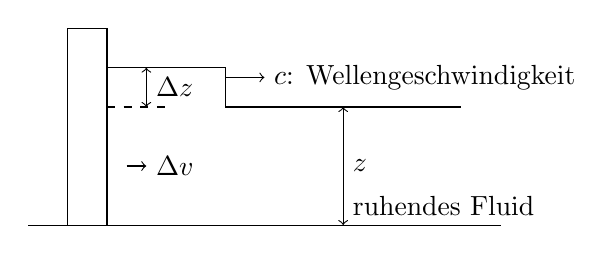
\begin{tikzpicture}
            \draw (0,0) -- (6,0);
            \draw (.5,0) rectangle (1,2.5);
            \draw (1,2) -- (2.5,2) -- (2.5,1.5) -- (5.5,1.5);
            \draw[dashed] (1,1.5) -- (1.75,1.5);
            \draw[<->] (1.5,2) -- (1.5,1.5) node[midway,right] {\(\Delta z\)};
            \draw[->] (1.25,.75) -- (1.5,.75) node[right] {\(\Delta v\)};
            \draw[<->] (4,0) -- (4,1.5) node[midway,right] {\(z\)};
            \node[anchor=south west] at (4,0) {ruhendes Fluid};
            \draw[->] (2.5,1.875) -- (3,1.875) node[right] {\(c\): Wellengeschwindigkeit};
        \end{tikzpicture}
    \end{center}
    aufweist.
    Im mit der Geschwindigkeit \(c\) mitbewegtem Bezugssystem wird die Strömung stationär wahrgenommen, rechts der Welle ist \(v = -c\), links \(v = -c + \Delta v\).
    Zur Bestimmung von \(c\) greifen wir auf die Kontinuitätsgleichung und den Impulssatz zurück.
    \begin{center}
        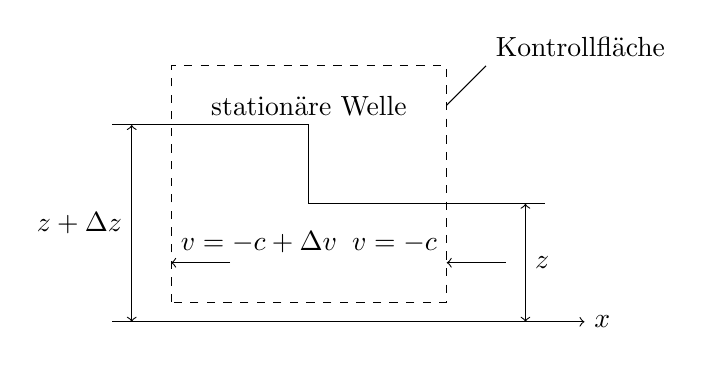
\begin{tikzpicture}
            \draw[->] (0,0) -- (6,0) node[right] {\(x\)};
            \draw (0,2.5) -- (2.5,2.5) -- (2.5,1.5) -- (5.5,1.5);
            \draw[<->] (.25,0) -- (.25,2.5) node[midway,left] {\(z + \Delta z\)};
            \draw[<->] (5.25,0) -- (5.25,1.5) node[midway,right] {\(z\)};
            \draw[dashed] (.75,.25) rectangle (4.25,3.25);
            \draw[->] (1.5,.75) -- (.75,.75);
            \node[anchor=south west] at (.75,.75) {\(v = -c + \Delta v\)};
            \draw[->] (5,.75) -- (4.25,.75) node[above left] {\(v = -c\)};
            \node[anchor=south] at (2.5,2.5) {stationäre Welle};
            \draw (4.25,2.75) -- (4.75,3.25) node[above right] {Kontrollfläche};
        \end{tikzpicture}
    \end{center}
    Bei uniformer eindimensionaler Strömung ergibt die Erhaltung der Masse
    \[
        -czb = \parentheses*{-c + \Delta v}\parentheses*{z + \Delta z}b,
    \]
    wobei \(b\) die Kanalbreite ist.
    Daraus ergibt sich
    \[
        c = \frac{\parentheses*{z + \Delta z}\Delta v}{\Delta z}
    \]
    bzw. für Wellen geringer Amplitude \(\Delta z \ll z\)
    \[
        c = z\frac{\Delta v}{\Delta z}.
    \]
    Der Impulssatz besagt
    \begin{align*}
        p_a bz_{\Delta}' + \int_0^{z + \Delta z}\parentheses*{p_a + \rho gz}b\d z - p_a bz' - \int_0^z \parentheses*{p_a + \rho gz}b\d z &= \rho cbz\parentheses*{-c + \Delta v + c}\\
        \iff \frac{1}{2}\rho gbz^2 - \frac{1}{2}\rho gb\parentheses*{z + \Delta z}^2 &= -\rho cbz\Delta v.
    \end{align*}
    Bedenkt man
    \[
        \Delta z^2 \ll z\Delta z,
    \]
    so folgt
    \[
        \frac{\Delta v}{\Delta z} = \frac{g}{c}
    \]
    bzw.
    \[
        c^2 = gz.
    \]
    Somit lautet die Geschwindigkeit einer Welle kleiner Aplitude
    \[
        c = \sqrt{gz}.
    \]
    Sie ist unabhängig von der Dichte des Fluids, jedoch abhängig von der Erdbeschleunigung \(g\), da eine derartige Wellenbewegung aus einem Gleichgewicht zwischen Trägheitseffekten, die zu \(\rho\) proportional sind, und Gewichtseffekten, die sich proportional zu \(\rho g\) verhalten, besteht.
    Ein Verhältnis dieser Kräfte enthält somit lediglich \(g\).


    \subsection*{Strömungsformen der Gerinneströmung}

    In obiger Betrachtung sind wir davon ausgegangen, dass sich eine Welle in einem ruhenden Fluid mit einer Geschwindigkeit \(c\) relativ zum Fluid und zu einem festen Beobachter rechtslaufend ausbreitet.
    Strömt das Fluid mit einer Geschwindigkeit \(v < c\) nach links, bewegt sich die Welle für einen ruhenden Beobachter mit einer Geschwindigkeit \(c - v\) nach rechts.
    Im Falle \(v = c\) ruht die Welle und für \(v > c\) wandert die Welle mit \(v - c\) nach links.

    Dieser Zusammenhang kann auch mittels der Frondezahl \(Fr\), die das Verhältnis von Fluid- und Wellengeschwindigkeit darstellt \(Fr = \frac{v}{c} = \frac{v}{\sqrt{gz}}\) ausgedrückt werden.
    Zur Wellenerzeugung wird ein Stein in einem FLuss geworfen.
    Sofern keine Strömung vorliegt, breitet sich die Welle in sämtliche Richtungen aus.
    Ist die Fließgeschwindigkeit \(v < c\), kann die Welle stromauf wandern.
    Das heißt ein Beobachter stromauf der Strömung, die durch den Stein erzeugt wird, nimmt diese wahr, er wird von ihr beinflusst.
    Derartige Strömungen mit \(v < c\) bzw. \(Fr < 1\) werden als unterkritisch bezeichnet.
    Demgegenüber stehen die überkritischen Strömungen, in denen die Strömungsgeschwindigkeit größer als die Wellengeschwindigkeit ist \(v > c\) bzw. \(Fr > 1\).
    In ihnen werden Strömungen stromauf nicht festgestellt, sie wandern alle stromab.
    Ist \(v = c\) bzw. \(Fr = 1\) spricht man von einer kritischen Strömung.

    Der Charakter der offenen Gerinneströmung hängt stark davon ab, ob sie unter- oder überkritisch ist.
    So kann z.B. eine Bodenwelle im Flussbett Ursache dafür sein, dass die Spiegelhöhe des Flusses unter diejenige absinkt, die ohne ``Strömung'' auftreten würde, oder sie könnte ein höheres Niveau aufweisen.
    Welche Strömung sich einstellt, hängt von der Froudezahl ab.
    In überkritischen Strömungen können nahezu diskontinuierliche Tiefenänderungen auftreten, während in unterkritischen Strömungen die Veränderungen glatt und stetig verlaufen.

    Interessanterweise existieren gewisse Ähnlichkeiten zwischen der offenen Gerinneströmung einer Flüssigkeit und der kompressiblen Strömung eines Gases.
    In beiden Fällen ist der entscheidende Parameter ein Verhältnis aus Fluidgeschwindigkeit und Wellengeschwindigkeit; im Falle der Gerinneströmung wird die Ausbreitungsgeschwindigkeit der Oberflächenwellen herangezogen und bei der Analyse kompressibler Strömungen die Schallgeschwindigkeit.
    Viele der Differenzen zwischen unterkritischen (\(Fr < 1\)) und überkritischen (\(Fr > 1\)) Strömungen kaben Analoga in subsonischen (\(M < 1\)) und supersonischen (\(M > 1\)) Strömungen, wobei \(M\) der Machzahl, dem Verhältnis aus Fluidgeschwindigkeit und Schallgeschwindigkeit entspricht.


    \subsection*{Energiehöhendiagramm}

    Die unterschiedlichen Strömungsformen können in einem Energiediagramm zusammengefasst werden.
    Dazu betrachten wir ein typisches Segment der offenen Gerinneströmung.
    Die Steigung der Sohle ist \(s_0 = \frac{y_1 - y_2}{l}\), sie ist in den meisten offenen Gerinneströmungen sehr klein.

    Berücksichtigt man ein uniformes Geschwindigkeitsprofil, ergibt die eindimensionale Energiegleichung
    \[
        z_1 + \frac{v_1^2}{2g} + s_0 l = z_2 + \frac{v_2^2}{2g} + h_v,
    \]
    wobei \(h_v\) einen Verlustterm darstellt, der als \(s_v l\) geschrieben werden kann.
    Somit ist
    \[
        z_1 - z_2 = \frac{v_2^2 - v_1^2}{2g} + \parentheses*{s_v - s_0}l.
    \]
\end{document}
